\documentclass[tikz,border=6pt]{standalone}
% Shared preamble of the standalone figures: fonts as in the decks, the TikZ
% libraries, the notation, and the styles.
\usepackage[T1]{fontenc}
\usepackage[utf8]{inputenc}
\usepackage[sfdefault,lining]{FiraSans}
\usepackage{FiraMono}
\usepackage{amsmath}
\usetikzlibrary{positioning,arrows.meta,calc,shapes.misc,fit,backgrounds,
                decorations.pathreplacing,patterns,matrix}
% Notation for the MACE4D figures.
%
% Every parameter, symbol, default value, and constant that a figure shows is
% a macro here, so that the figures change from code names to symbols, or
% follow a change of a default, by editing this file alone.
%
%   \codenamestrue   renders each parameter as its code name (current setting)
%   \codenamesfalse  renders the symbolic form
%
% \sym{code name}{symbol} is the switch every parameter macro uses.  A
% parameter that exists on both models carries its owner in code mode.

\newif\ifcodenames
\codenamestrue

\providecommand{\code}[1]{\texttt{#1}}
\newcommand{\sym}[2]{\ifcodenames\code{#1}\else\ensuremath{#2}\fi}
\newcommand{\ctmodel}{\code{ct\_model}}
\newcommand{\macemodel}{\code{MACE4DModel}}
% A key line "code name <-> symbol", shown in code mode only.
\newcommand{\keyline}[2]{\ifcodenames#1~\ensuremath{\leftrightarrow}~\ensuremath{#2}\fi}

% ------------------------------------------------------------ math symbols
% These are always symbolic; the formulas use them, and the key lines tie
% them to the code names.
\newcommand{\symSigY}{\sigma_y}
\newcommand{\symSigProx}{\sigma_p}
\newcommand{\symSigNoise}{\sigma_n}
\newcommand{\symSigX}{\sigma_x}
\newcommand{\symSharpness}{s}
\newcommand{\symBeta}[1]{\beta_{#1}}
\newcommand{\symRho}{\rho}
\newcommand{\symNbrWeightTime}{b_t}
\newcommand{\symNumFrames}{T}
\newcommand{\symFramesPerRotation}{P}
\newcommand{\symOverlap}{f}

% ------------------------------------------------------------------ objects
\newcommand{\frameCube}[1]{\ensuremath{C_{#1}}}          % frame t of the 4D image
\newcommand{\fourD}{\ensuremath{x}}                      % the 4D image
\newcommand{\initImage}{\ensuremath{x^{0}}}              % the initial 4D image
\newcommand{\sinoFrame}[1]{\ensuremath{y_{#1}}}          % the views of frame t
\newcommand{\weightsFrame}[1]{\ensuremath{\Lambda_{#1}}} % the weights of frame t
\newcommand{\projFrame}[1]{\ensuremath{A_{#1}}}          % the frame model
\newcommand{\proxAgent}[1]{\ensuremath{F_{#1}}}          % the prox map of frame t
\newcommand{\dataFitAgent}{\ensuremath{F}}               % all frames' prox maps as one agent
\newcommand{\orientXY}{\sym{XY-t}{\mathrm{XY}t}}
\newcommand{\orientYZ}{\sym{YZ-t}{\mathrm{YZ}t}}
\newcommand{\orientXZ}{\sym{XZ-t}{\mathrm{XZ}t}}
\newcommand{\denoiser}[1]{\ensuremath{G_{#1}}}           % \denoiser{\orientXY}
\newcommand{\stateW}[1]{\ensuremath{W_{#1}}}             % the loop's input to agent k
\newcommand{\outX}[1]{\ensuremath{X_{#1}}}               % the output of agent k
\newcommand{\avgZ}{\ensuremath{z}}
\newcommand{\xbar}{\ensuremath{\bar{x}}}
\newcommand{\filterMatrix}{\sym{filter\_matrix}{H}}
\newcommand{\genInit}{\code{'init'}}                     % the generator of the partitions
\newcommand{\genIteration}{the iteration number}          % the generator of the subset order

% --------------------------------------------- parameters and their defaults
% Scan and frames (constructor arguments of MACE4DModel)
\newcommand{\pFramesPerRotation}{\sym{frames\_per\_rotation}{\symFramesPerRotation}}
\newcommand{\defFramesPerRotation}{6}
\newcommand{\pFrameOverlapFactor}{\sym{frame\_overlap\_factor}{\symOverlap}}
\newcommand{\defFrameOverlapFactor}{2.0}
\newcommand{\pNumFrames}{\sym{num\_frames}{\symNumFrames}}
\newcommand{\defNumFrames}{all}

% Set on ct_model; reach the frame models
\newcommand{\pSnrDb}{\sym{snr\_db}{\mathrm{SNR}_{\mathrm{dB}}}}
\newcommand{\defSnrDb}{30}
\newcommand{\pSharpnessCt}{\sym{ct\_model.sharpness}{\symSharpness_{\mathrm{ct}}}}
\newcommand{\defSharpnessCt}{1.0}
\newcommand{\pSigmaProxCt}{\sym{ct\_model.sigma\_prox}{\symSigProx^{\mathrm{ct}}}}
\newcommand{\pSigmaXCt}{\sym{ct\_model.sigma\_x}{\symSigX^{\mathrm{ct}}}}
\newcommand{\pPQTCt}{\sym{ct\_model.p, q, T}{(p, q, T)_{\mathrm{ct}}}}
\newcommand{\pSigmaY}{\sym{sigma\_y}{\symSigY}}

% Set on MACE4DModel
\newcommand{\pSigmaProxMace}{\sym{MACE4DModel.sigma\_prox}{\symSigProx}}
\newcommand{\defSigmaProxMace}{None (estimated per frame)}
\newcommand{\pSigmaNoise}{\sym{sigma\_noise}{\symSigNoise}}
\newcommand{\defSigmaNoise}{None (estimated)}
\newcommand{\pSigmaXMace}{\sym{MACE4DModel.sigma\_x}{\symSigX}}
\newcommand{\defSigmaXMace}{estimated}
\newcommand{\pSharpnessMace}{\sym{MACE4DModel.sharpness}{\symSharpness}}
\newcommand{\defSharpnessMace}{0.0}
\newcommand{\pPQTMace}{\sym{MACE4DModel.p, q, T}{(p, q, T)}}
\newcommand{\defPQT}{2.0, 1.2, 1.0}
\newcommand{\pNbrWeightTime}{\sym{nbr\_weight\_time}{\symNbrWeightTime}}
\newcommand{\defNbrWeightTime}{1.0}
\newcommand{\pMacePriorWeight}{\sym{mace\_prior\_weight}{\beta}}
\newcommand{\defMacePriorWeight}{0.5}
\newcommand{\pRhoMann}{\sym{rho\_mann}{\symRho}}
\newcommand{\defRhoMann}{0.5}
\newcommand{\pProxNumIterations}{\sym{prox\_num\_iterations}{N_p}}
\newcommand{\defProxNumIterations}{3}
\newcommand{\pProxPartitionAdvance}{\sym{prox\_partition\_advance}{a}}
\newcommand{\defProxPartitionAdvance}{1.0}
\newcommand{\pProxWarmStart}{\code{prox\_warm\_start}}
\newcommand{\defProxWarmStart}{True}
\newcommand{\pProxStopThreshold}{\code{prox\_stop\_threshold}}
\newcommand{\defProxStopThreshold}{0.02}
\newcommand{\pDenoiserWarmStart}{\code{denoiser\_warm\_start}}
\newcommand{\defDenoiserWarmStart}{False}
\newcommand{\pDenoiseSlabGb}{\code{denoise\_slab\_gb}}
\newcommand{\defDenoiseSlabGb}{2.0}
\newcommand{\pDejitter}{\code{dejitter}}
\newcommand{\defDejitter}{True}
\newcommand{\pDevicePool}{\code{set\_device\_pool}}
\newcommand{\pNumDevicesEnv}{\code{MBIRTORCH\_NUM\_DEVICES}}

% Arguments of MACE4DModel.recon
\newcommand{\pMaxIterations}{\sym{max\_iterations}{N}}
\newcommand{\defMaxIterations}{10}
\newcommand{\pStopThreshold}{\code{stop\_threshold\_change\_pct}}
\newcommand{\defStopThreshold}{0.2}
\newcommand{\pSeed}{\code{seed}}
\newcommand{\defSeed}{None}
\newcommand{\pInitRecon}{\code{init\_recon}}
\newcommand{\pInitDir}{\code{init\_dir}}

% ---------------------------------------------------------------- constants
\newcommand{\cInitIterations}{15}        % iterations of the per-frame initial image
\newcommand{\cDenoiseMaxIterations}{15}  % iterations per denoised volume, at most
\newcommand{\cDenoiseStopPct}{0.05}      % percent change that stops a denoised volume
\newcommand{\cSigmaXFactor}{0.2}         % sigma_x and sigma_prox estimates: factor * 2^sharpness * std
\newcommand{\cSigmaXFloor}{10^{-6}}      % floor of the denoiser sigma_x estimate
\newcommand{\cSigmaXBase}{1.0}           % base default of sigma_x when no estimate runs
\newcommand{\cDenoiseSubsets}{16}        % pixel subsets of a denoiser partition, at most
\newcommand{\cPixelsPerSubset}{64}       % fewer pixels per subset than this and the count drops

% ------------------------------------------- symbols the figures use inline
\newcommand{\symPriorWeight}{\ensuremath{w}}    % the value of the prior weight
\newcommand{\symFilterMatrix}{\ensuremath{H}}   % the temporal filter
\newcommand{\symFrameIndex}{\ensuremath{t}}
\newcommand{\symNumDevices}{\ensuremath{n}}     % the size of the device pool
\newcommand{\degsym}{\ensuremath{^{\circ}}}
% Argument values of the device pool selector
\newcommand{\valNone}{\code{None}}
\newcommand{\valCpu}{\code{'cpu'}}
\newcommand{\valGpu}{\code{'gpu'}}
% Derived defaults, in degrees (integers; add rounding if a default ever gives a fraction)
\newcommand{\defFrameStepDeg}{\pgfmathparse{int(360/\defFramesPerRotation)}\pgfmathresult}
\newcommand{\defFrameSpanDeg}{\pgfmathparse{int(\defFrameOverlapFactor*360/\defFramesPerRotation)}\pgfmathresult}
% Axis labels of the 4D image
\newcommand{\axisT}{\ensuremath{t}}
\newcommand{\axisX}{\ensuremath{x}}
\newcommand{\axisY}{\ensuremath{y}}
\newcommand{\axisZ}{\ensuremath{z}}

% Colors and TikZ styles shared by the MACE4D figures.
%
% Blue is the data-fit side, green the priors, amber the consensus state.
% A solid arrow carries a value the user set; a dashed arrow carries an
% estimate.  \cube draws one frame of the 4D image.

\definecolor{datafitBlue}{HTML}{3D6B99}
\definecolor{priorGreen}{HTML}{2E7D32}
\definecolor{stateAmber}{HTML}{B26B1F}
\definecolor{warnRed}{HTML}{A23B3B}
\definecolor{inkGray}{HTML}{5A5A5A}
\definecolor{lineGray}{HTML}{9A9A9A}
\definecolor{paleBlue}{HTML}{E3ECF5}
\definecolor{paleGreen}{HTML}{E4F0E4}
\definecolor{paleAmber}{HTML}{F5EBDD}
\definecolor{paleGray}{HTML}{F0F0F0}

\tikzset{
  every node/.style={font=\small},
  box/.style={draw, rounded corners=3pt, thick, align=center, inner sep=5pt,
              minimum height=8mm},
  datafit/.style={box, draw=datafitBlue, fill=paleBlue},
  prior/.style={box, draw=priorGreen, fill=paleGreen},
  state/.style={box, draw=stateAmber, fill=paleAmber},
  plain/.style={box, draw=lineGray, fill=paleGray},
  note/.style={font=\footnotesize, text=inkGray, align=left},
  notebox/.style={note, draw=lineGray, rounded corners=2pt, inner sep=4pt,
                  fill=white},
  param/.style={font=\footnotesize, align=left},
  title/.style={font=\bfseries, align=left},
  setarrow/.style={-{Stealth[length=2mm]}, thick},
  estarrow/.style={-{Stealth[length=2mm]}, thick, dashed, inkGray},
  flow/.style={-{Stealth[length=2mm]}, semithick},
  flowblue/.style={flow, datafitBlue},
  flowgreen/.style={flow, priorGreen},
  flowamber/.style={flow, stateAmber},
  cut/.style={-{Stealth[length=1.5mm]}, thin, inkGray},
  cubeFront/.style={fill=white, draw=black!70, thin},
  cubeTop/.style={fill=black!8, draw=black!70, thin},
  cubeSide/.style={fill=black!20, draw=black!70, thin},
}

% \cube{x}{y}{size}{label}: a cube whose front face has its lower left
% corner at (x, y) and side length size, with a label on the front face.
\newcommand{\cube}[4]{%
  \begin{scope}[shift={(#1,#2)}]
    \pgfmathsetmacro{\cubeDepth}{0.35*#3}
    \draw[cubeTop] (0,#3) -- (\cubeDepth,#3+\cubeDepth) -- (#3+\cubeDepth,#3+\cubeDepth) -- (#3,#3) -- cycle;
    \draw[cubeSide] (#3,0) -- (#3+\cubeDepth,\cubeDepth) -- (#3+\cubeDepth,#3+\cubeDepth) -- (#3,#3) -- cycle;
    \draw[cubeFront] (0,0) rectangle (#3,#3);
    \node at (0.5*#3,0.5*#3) {#4};
  \end{scope}}

% \arrowkey{x}{y}: the legend of the two arrow kinds, anchored at (x, y).
\newcommand{\arrowkey}[2]{%
  \draw[setarrow] (#1,#2) -- ++(1,0) node[note, right] {set by the user};
  \draw[estarrow] (#1,#2-0.45) -- ++(1,0) node[note, right] {estimated from the data};}



% Labels break between words, never inside one.
\hyphenpenalty=10000
\exhyphenpenalty=10000
\tolerance=9999
\emergencystretch=1em

% The second line of a parameter box, which carries its default.
\newcommand{\defline}[1]{\\[1pt]{\scriptsize #1}}
% \cutbar{x}{y}: the mark that stops an estimate where a set value takes over.
\newcommand{\cutbar}[2]{%
  \draw[line width=1.1pt, inkGray] ({#1-0.08},{#2-0.26}) -- ({#1-0.08},{#2+0.26});
  \draw[line width=1.1pt, inkGray] ({#1+0.08},{#2-0.26}) -- ({#1+0.08},{#2+0.26});}

% The three bands of each column, and the label of an arrow that takes over.
\tikzset{
  pbox/.style={text width=3.75cm, font=\footnotesize},
  ebox/.style={plain, text width=3.1cm, font=\footnotesize},
  sbox/.style={text width=1.95cm, font=\footnotesize},
  tbox/.style={text width=3.1cm, font=\footnotesize},
  wins/.style={font=\footnotesize\bfseries, fill=white, inner sep=1.5pt},
  winarrow/.style={setarrow, line width=1.1pt},
}

\begin{document}
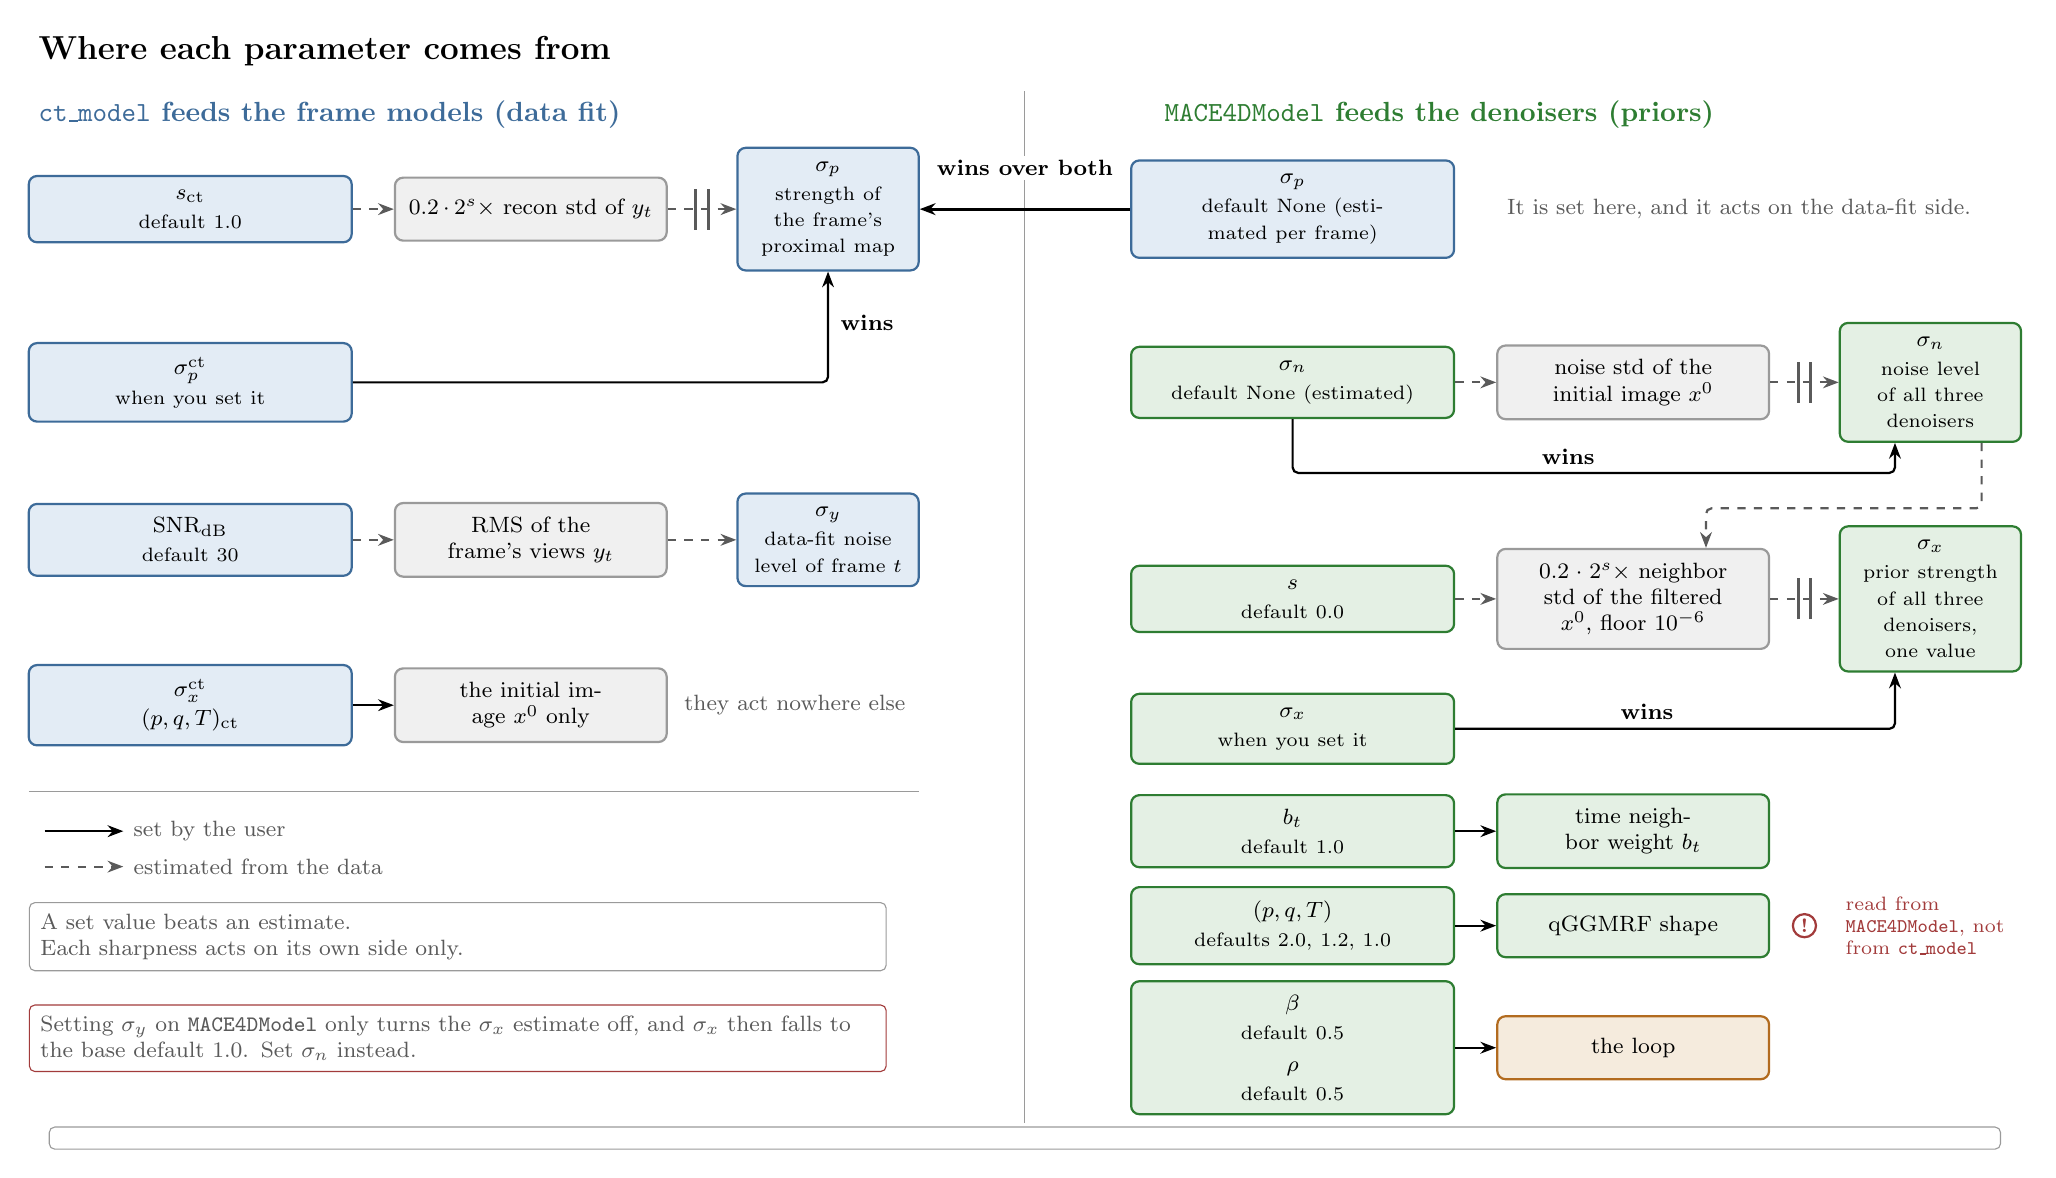
\begin{tikzpicture}

% ---------------------------------------------------- title and the two columns
\node[title, font=\large\bfseries, anchor=west] at (-12.65,2.9) {Where each parameter comes from};
\node[title, text=datafitBlue, anchor=west] at (-12.65,2.1)
  {\ctmodel{} feeds the frame models (data fit)};
\node[title, text=priorGreen, anchor=west] at (1.65,2.1)
  {\macemodel{} feeds the denoisers (priors)};
\draw[lineGray] (0,2.4) -- (0,-10.7);

% ------------------------------------------ left column: the proximal strength
\node[datafit, pbox] (pshct) at (-10.6,0.9)
  {\pSharpnessCt\defline{default \defSharpnessCt}};
\node[ebox] (eprox) at (-6.275,0.9)
  {$\cSigmaXFactor \cdot 2^{\symSharpness} \times$ recon std of \sinoFrame{t}};
\node[datafit, sbox] (sprox) at (-2.5,0.9)
  {$\symSigProx$\defline{strength of the frame's proximal map}};
\draw[estarrow] (pshct) -- (eprox);
\draw[estarrow] (eprox) -- (sprox);
\cutbar{-4.1}{0.9}

% the value set on ct_model, which stops that estimate
\node[datafit, pbox] (pproxct) at (-10.6,-1.3)
  {\pSigmaProxCt\defline{when you set it}};
\draw[setarrow, rounded corners=2pt]
  (pproxct.east) -- (-2.5,-1.3) -- (sprox.south);
\node[wins, anchor=west] at (-2.4,-0.55) {wins};

% ---------------------------------------- left column: the data-fit noise level
\node[datafit, pbox] (psnr) at (-10.6,-3.3)
  {\pSnrDb\defline{default \defSnrDb}};
\node[ebox] (esigy) at (-6.275,-3.3)
  {RMS of the frame's views \sinoFrame{t}};
\node[datafit, sbox] (ssigy) at (-2.5,-3.3)
  {$\symSigY$\defline{data-fit noise level of frame $t$}};
\draw[estarrow] (psnr) -- (esigy);
\draw[estarrow] (esigy) -- (ssigy);

% ------------------------------------ left column: the two that reach only x0
\node[datafit, pbox] (pinit) at (-10.6,-5.4) {\pSigmaXCt\\[1pt]\pPQTCt};
\node[ebox] (einit) at (-6.275,-5.4) {the initial image \initImage{} only};
\draw[setarrow] (pinit) -- (einit);
\node[note, anchor=west] at (-4.45,-5.4) {they act nowhere else};

% ------------------- right column: the one value that crosses to the other side
\node[datafit, pbox] (pproxmace) at (3.4,0.9)
  {\pSigmaProxMace\defline{default \defSigmaProxMace}};
\draw[winarrow] (pproxmace.west) -- (sprox.east);
\node[wins] at (0,1.42) {wins over both};
\node[note, anchor=west, text width=6.3cm] at (6.0,0.9)
  {It is set here, and it acts on the data-fit side.};

% ---------------------------------------- right column: the denoiser noise level
\node[prior, pbox] (pnoise) at (3.4,-1.3)
  {\pSigmaNoise\defline{default \defSigmaNoise}};
\node[ebox] (esign) at (7.725,-1.3)
  {noise std of the initial image \initImage};
\node[prior, sbox] (ssign) at (11.5,-1.3)
  {$\symSigNoise$\defline{noise level of all three denoisers}};
\draw[estarrow] (pnoise) -- (esign);
\draw[estarrow] (esign) -- (ssign);
\cutbar{9.9}{-1.3}
\draw[setarrow, rounded corners=2pt] (pnoise.south) -- (3.4,-2.45)
  -- (11.05,-2.45) -- ($(ssign.south)-(0.45,0)$);
\node[wins, above=1.5pt] at (6.9,-2.45) {wins};

% -------------------------------------------- right column: the prior strength
\node[prior, pbox] (pshmace) at (3.4,-4.05)
  {\pSharpnessMace\defline{default \defSharpnessMace}};
\node[ebox] (esigx) at (7.725,-4.05)
  {$\cSigmaXFactor \cdot 2^{\symSharpness} \times$ neighbor std of the filtered
   \initImage, floor $\cSigmaXFloor$};
\node[prior, sbox] (ssigx) at (11.5,-4.05)
  {$\symSigX$\defline{prior strength of all three denoisers, one value}};
\draw[estarrow] (pshmace) -- (esigx);
\draw[estarrow] (esigx) -- (ssigx);
\cutbar{9.9}{-4.05}
% the noise level is the estimator's second input
\draw[estarrow, rounded corners=2pt] ($(ssign.south)+(0.65,0)$) -- (12.15,-2.9)
  -- (8.65,-2.9) -- ($(esigx.north)+(0.925,0)$);

% the value set on MACE4DModel, which stops that estimate
\node[prior, pbox] (psigxmace) at (3.4,-5.7)
  {\pSigmaXMace\defline{when you set it}};
\draw[setarrow, rounded corners=2pt] (psigxmace.east) -- (11.05,-5.7)
  -- ($(ssigx.south)-(0.45,0)$);
\node[wins, above=1.5pt] at (7.9,-5.7) {wins};

% -------------------------------- right column: the values that are used as set
\node[prior, pbox] (pnbr) at (3.4,-7.0)
  {\pNbrWeightTime\defline{default \defNbrWeightTime}};
\node[prior, tbox] (tnbr) at (7.725,-7.0) {time neighbor weight $\symNbrWeightTime$};
\draw[setarrow] (pnbr) -- (tnbr);

\node[prior, pbox] (ppqt) at (3.4,-8.2) {\pPQTMace\defline{defaults \defPQT}};
\node[prior, tbox] (tpqt) at (7.725,-8.2) {qGGMRF shape};
\draw[setarrow] (ppqt) -- (tpqt);
\node[circle, draw=warnRed, fill=white, thick, inner sep=1pt,
      font=\scriptsize\bfseries, text=warnRed] at (9.9,-8.2) {!};
\node[note, text=warnRed, anchor=west, text width=2.2cm, font=\scriptsize]
  at (10.3,-8.2) {read from \macemodel{}, not from \ctmodel};

\node[prior, pbox] (ploop) at (3.4,-9.75)
  {\pMacePriorWeight\defline{default \defMacePriorWeight}\\[2pt]
   \pRhoMann\defline{default \defRhoMann}};
\node[state, tbox] (tloop) at (7.725,-9.75) {the loop};
\draw[setarrow] (ploop) -- (tloop);

% ------------------------------------------------- the key and the two warnings
\draw[lineGray, thin] (-12.65,-6.5) -- (-1.35,-6.5);
\arrowkey{-12.45}{-7.0}
\node[notebox, anchor=north west, text width=10.6cm] at (-12.65,-7.9)
  {A set value beats an estimate.\\
   Each sharpness acts on its own side only.};
\node[notebox, anchor=north west, text width=10.6cm, draw=warnRed] at (-12.65,-9.2)
  {Setting \pSigmaY{} on \macemodel{} only turns the $\symSigX$ estimate off,
   and $\symSigX$ then falls to the base default \cSigmaXBase.
   Set \pSigmaNoise{} instead.};

% ------------------------------------------------------- code names and symbols
\node[notebox, anchor=north, text width=24.5cm, align=center] at (0,-10.75)
  {\keyline{\pSigmaY}{\symSigY} \quad
   \keyline{\pSigmaProxMace}{\symSigProx} \quad
   \keyline{\pSigmaNoise}{\symSigNoise} \quad
   \keyline{\pSigmaXMace}{\symSigX} \quad
   \keyline{\pSharpnessMace}{\symSharpness}};

\end{tikzpicture}
\end{document}
